%-------------------------------------------------------------------------
\section{Research Overview, Motivations and Objectives}\label{sec:intro}
%-------------------------------------------------------------------------

Tele-operated robotic systems enable workers to perform manufacturing and maintenance tasks in remote, inaccessible, and/or hazardous environments. Complex and risk-sensitive tasks that require dexterous motion coordination skills and decision-making intelligence cannot be fully automated, yet can be reliably accomplished under human control. Given a specific task and robotic system, the performance of human-robot teleoperation depends on the usability of the teleoperation interface and the teleoperator'expertise. The state-of-the-art robotic systems, including humanoid and multi-robot systems, have been endowed with the motion capabilities that conventional teleoperation interfaces cannot fully utilize. Teleoeprating such robotic systems are particularly difficult when the tasks involve mutli-component, multi-arm and multi-robot coordination. Given the complexity of robotic systems and tasks, novel measurement metrics for interface usability and human performance need to be developed to inform the teleoperation interface design and teleoperation skill development for complex robot motion coordination. 

% Metrics for human performance in simple tasks are not sufficient to evaluate the teleoperation skill of  

% Previous research have proposed novel teleoperation interface design that facilitate intuitive motion/perception mapping, and reduce physical and cognitive workload and discomfort.

To meet this need, we propose a novel perspective to understand the performance of human-robot teleoperation. We propose a hierarchical framework to \underline{model the structure of teleoperated robot motion}, such that the evaluation of low-level motor skill can be separated from that of high-level task planning. Based on this framework, we propose novel metrics, including \textit{Outcome Predictability}, \textit{Mapping Sensitivity}, \textit{Operation complexity}, to \underline{measure the usability of teleoperation interfaces}. These metrics evaluates the robot control interface's capabilities of mapping the low-level motor skill and high-level task plan from human to the controlled robotic systems. We use these metrics to compare several conventional and novel control interfaces for a mobile humanoid robot (see \fig{NursingTask}), in general-purpose tasks that involve arm-hand coordination, bimanual coodination, loco-manipulation, and human-robot collaboration. 

% \begin{wrapfigure}{r}{0.75\linewidth}
\begin{figure}[h!!]
\centering
% \vspace{0.8ex}
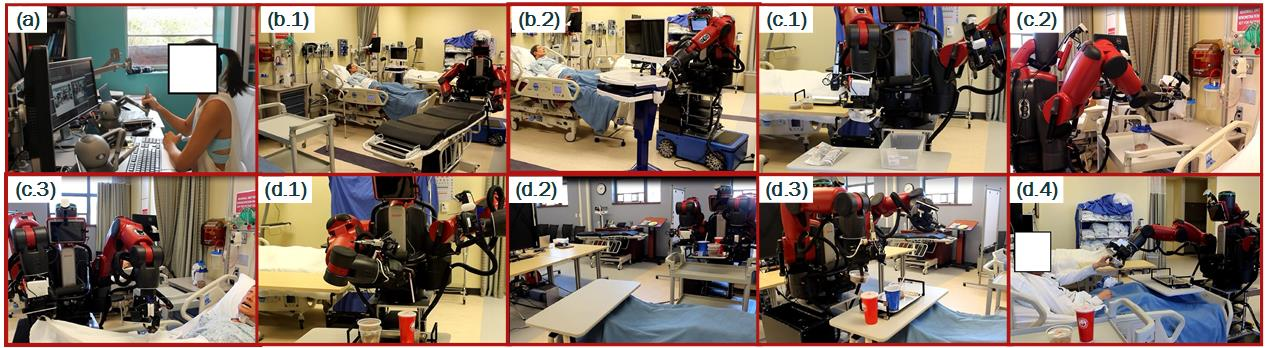
\includegraphics[width=0.99\linewidth]{fig//NursingTask}
\caption{Under (a) direct teleoperation, a mobile humanoid robot tasks can perform complex nursing tasks, including (b.1-2) moving a portable medical devices; (c.1-3) organizing and cleaning the patient's room; and (d.1-4) preparing and serving food to a patient. The manipulation and/or locomotion coordination involved is shared across warehouse, social and in-home assistance scenarios. }
\label{NursingTask}
\vspace{1ex}
\end{figure}
% \end{wrapfigure}

We further propose a novel approach to \underline{evaluate human skill progression} in the training of using different teleoperation interfaces. Our approach grounds in Bernstein's observation that the characteristics that distinguish an expert motor skill are the strong motion regularity that reflects the performance optimization resulted from sufficient practice and refinement, and a small variability to render flexible behavior in the presence of uncertainty. For each teleoperation interface, we extract the motion primitives and task plan of the teleoperated motion coordination, and study their evolution as the teleoperator's skill progresses from novice to expert. Across different teleoperation interfaces, We compare how the teleoperators discover, refine, merge and purge the set of motion primitives and reshape their high-level task plans accordingly. After the teleopertator's skill converge to stable policy and task performance, we further compare the motion coordination strategies in the control of human body and robotic embodiment, to infer the reward function for teleoperated motion coordination. 

This 1-year project will conduct the following three research tasks: 

\begin{itemize}

\item \textbf{Task 1} --- Modeling complex motion coordination of teleoperated robots

% Develop a novel framework to decompose motion coordination to low-level motor skills and high-level task plan; propose modeling methods for coordinated motion primitives and task plan for single robot task and human-robot interaction.   

\item \textbf{Task 2} --- Collecting robot teleoperation data for general-purpose motion coordination tasks  

% Propose novel measurement metrics for evaluating the motion mapping capability of teleoperation interfaces; Compare various teleoperation interfaces for controlling a mobile humanoid to perform general-purpose warehouse tasks that involve complex motion coordination. 

\item \textbf{Task 3} --- Evaluating interface motion mapping capability and teleoperation skill

% Propose novel human performance metrics to evaluate low-level motor skills and high-level task planning skills; study the teleoperation skill progression 

% Develop performance evaluation metrics for human-robot teleoperation system; Study the progression of teleoperated motion coordination from novice to expert, and identify the milestones and thresholds of performance improvement; Investigate the evolution of motion primitives and task plan; Prescribe multi-modality cognitive augmentation to overcome the skill development thresholds; Prescribe physical-cognitive training tasks to develop transferable skills for perception-motion coordination. 

\end{itemize}

\paragraph*{Intellectual Merits}
The intellectual merit of this proposal includes contributions to performance measurement of human-robot collaboration in the teleoperation of complex robotic systems. It proposes a novel measurement framework for evaluating human performance of high-level decision-making and low-level motor skill. It also addresses a critical need in human-robot interface design for evaluation metrics that can quantitatively compare the motion mapping transparency and complexity.

\paragraph*{Broad Impacts}
This project will benefit the teleoperation interface design and evaluation of a broad range of complex robotic systems for warehouse, manufacturing, and maintenance applications. The proposed framework for motion decomposition and performance metrics can be generally applied to measure the worker skill level and progress for industrial, medical, assistance, construction and military tasks, and can be extended to evaluate human skill progression in motor learning and recovery. This project will support one PhD student as research assistant for one year, and one graduate student for 3-month summer research. The research effort will be synergized with graduate and undergraduate courses and develop open-source intuitive teleoperation interface for mobile manipulator robots.  This project will also also involve a team of senior undergrad students working on major qualifying project (MQP), and engage K-12 students through First Robotics and general public in the annually Touch Tomorrow event at WPI.

 
\paragraph*{Qualification of Investigators}
PI Zhi Li has significant experience in tele-robotic systems, including exoskeletons for rehabilitation, tele-surgical robots and tele-nursing robots. Her research focuses on the modeling, planning and learning of complex human and robotic motion coordination, and extended on mechanical design optimization~\cite{li2016design}, robot system integration~\cite{Hauser_Li_TRINA:17}, networked haptics~\cite{li2009networked,li2009remote}, and physical human-robot interaction~\cite{Hauser_Li_BiTelepresence:17}. Related to the proposed project, she has developed the Tele-robotic Intelligent Nursing Assistant (TRINA) system with multi-modal teleoperation interfaces, and conducted system capability evaluation for the direct teleoperation of nursing tasks~\cite{Hauser_Li_TRINA:17}. She is an expert in the regularity and variability of human motion coordination, and human-inspired strategies for controlling kinematically of complex robotic systems~\cite{kim2012resolving,Rosen_Li_EMBC:13,Rosen_Li_IROSChapt:13,Rosen_Li_IROS:14,Rosen_Li_J:14, Rosen_Li:17}. Li's motion learning and prediction algorithm can resolve the kinematic redundancy of a dual-arm rehabilitation exoskeleton, enable it to render arm postures that are fully compatible with healthy operators, and correct abnormal joint coordination due to motor disability. She is also very knowledgeable in human motion skill meassurements~\cite{Rosen_Li_EMBC:15} and human performance in teleoperation~\cite{Hauser_Li_BiTelepresence:17}. 

